\begin{frame}
    \frametitle{Clave-Valor}

    Este modelo almacena pares del tipo (\textit{Key}, \textit{Value}).

    \begin{center}
    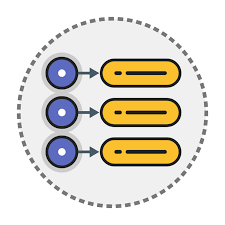
\includegraphics[width=0.2\textwidth]{diagramas/KeyValue.png}
    \end{center}
                    
     
        
     \begin{itemize}
        \item \textbf{Key}: Un identificador único para acceder al valor asociado.
         \item \textbf{Value}: Puede ser cualquier tipo de dato, desde texto, números y documentos, hasta listas o incluso otros pares clave-valor.
     
     \end{itemize}

\end{frame}

\begin{frame}
    \frametitle{Clave-Valor - Ventajas}
     \begin{itemize}
     
        \item No hay una estructura de tabla rígida, que permite esquemas flexibles.       
        
        \item Los campos pueden añadirse y modificarse dinámicamente sin alterar el esquema de la base de datos.
        
        \item Permiten el funcionamiento en clústeres, facilitando la adición de nodos para manejar grandes volúmenes de datos.
        
        \item Los motores de procesamiento en paralelo y la arquitectura de clústeres reducen los tiempos de consulta y mejoran la velocidad de escritura y lectura.
     
     \end{itemize}
\end{frame}


\begin{frame}
    \frametitle{Clave-Valor - Ejemplos}
    
    Algunas de las implementaciones más conocidas son:
    
     \begin{itemize}
        \item \textbf{Amazon DynamoDB}\\
        Una base de datos clave-valor y documental de Amazon Web Services. Ofrece alta escalabilidad y disponibilidad.
                        
         
        
        \item \textbf{Voldemort}\\
        Una base de datos distribuida impulsada por LinkedIn, diseñada para ofrecer alta disponibilidad y escalabilidad.
                        
         
        
        \item \textbf{Redis}\\
        Un proyecto de código abierto muy utilizado, especialmente para aplicaciones web modernas. Soporta estructuras de datos avanzadas como listas, sets y hashes.
                        
         
        
        \item \textbf{Riak}\\
        Un sistema escalable que facilita el desarrollo ágil de aplicaciones, con un enfoque en la simplicidad de uso.
     
     \end{itemize}
\end{frame}



% \section{Redis}
% \begin{frame}   
%     \frametitle{Clave-Valor - Redis}

%     \textbf{Redis} que significa ``\textbf{RE}mote \textbf{DI}ctionary \textbf{S}erver'', es una base de datos en memoria de código abierto.

%      

%     Si bien en la teoría, los valores son objetos oscuros, Redis ofrece estructuras de datos para los tipos tales como:

%      

%     \begin{enumerate}
%         \item \textit{Strings} (Valor simple)
%         \item \textit{Hashes}
%         \item \textit{Listas}
%         \item \textit{Conjuntos}
%         \item \textit{Conjuntos Ordenados}  
%         \item etc.
%     \end{enumerate}

%     Se pueden realizar operaciones \textbf{atómicas} sobre estas estructuras.
% \end{frame}

% \begin{frame}
%     \frametitle{Clave-Valor - Redis}
    
%     Redis ofrece más de \textbf{400} operaciones e implementa la interfaz teórica para cada uno de los tipos de datos mencionados (además de ofrecer otras operaciones).

%      

%     Algunos ejemplos son:

%      

%     \begin{itemize}
%         \item \textit{Strings:} $SET$, $GET$ y $DEL$

%          
        
%         \item \textit{Hashes:} $HSET$, $HGET$ y $HDEL$

%          
        
%         \item \textit{Listas:} $LPUSH$, $LPOP$, $RPUSH$, $RPOP$, $LRANGE$
%          

%         \item etc.
%     \end{itemize}

%      
    
%     La principal diferencia entre estas operaciones, es su complejidad temporal,   y hay que tenerla en cuenta.

%      

%     Hay que tener en claro el nivel de representatividad que se necesita, y capacidad de memoria que se posee, para elegir correctamente la estructura a utilizar.
% \end{frame}

% \begin{frame}[fragile]
%     \frametitle{Clave-Valor - Redis}
    
%     Algunos ejemplos de las operaciones mencionadas:

%      

%     \begin{verbatim}
%     redis> LPUSH mylist "NoSQL"
%     redis> LPUSH mylist "Datos" "De" "Bases"
%     redis> LRANGE mylist 0 2
%     1) "Bases"
%     2) "De"
%     3) "Datos"
%     redis>
%     \end{verbatim}

%      

%     \vspace{-0.8cm}
    
%     \begin{verbatim}
%     redis> ZADD myzset 2 "b" 3 "c"
%     (integer) 2
%     redis> ZADD myzset 4 "a"
%     redis> ZMEMBERS myset BYLEX
%     1) "a"
%     2) "b"
%     3) "c"
%     \end{verbatim}
    
% \end{frame}